\documentclass{hogent-article}
\usepackage{lipsum} % Voor vultekst
\usepackage{datetime} % Voor datums
\usepackage{enumitem} % Voor geletterde lijsten
\usepackage{placeins}

%------------------------------------------------------------------------------
% Metadata over het artikel
%------------------------------------------------------------------------------

%---------- Titel & auteur ----------------------------------------------------

\PaperTitle{Business analisten in agile werkomgevingen}
\PaperType{Hogeschool Gent | Business Analysis | Bedrijfscasus}
\Authors{Pieter Van de Walle\textsuperscript{1}, Noah Wallecan\textsuperscript{2}, Robbe Doeven\textsuperscript{3}, Musa Israïlov\textsuperscript{4}}
\newdate{date}{04}{12}{2022} % Zelf toegevoegd, .cls ook aangepast (lijn 205)
\CoPromotor{}

\affiliation{
  \textsuperscript{1} \href{mailto:pieter.vandewalle@student.hogent.be}{pieter.vandewalle@student.hogent.be}\newline
  \textsuperscript{2} \href{mailto:noah.wallecan@student.hogent.be}{noah.wallecan@student.hogent.be}\newline
  \textsuperscript{3} \href{mailto:robbe.doeven@student.hogent.be}{robbe.doeven@student.hogent.be}\newline
  \textsuperscript{4} \href{mailto:musa.israilov@student.hogent.be}{musa.israilov@student.hogent.be}
  }

%---------- Abstract ----------------------------------------------------------

\Abstract{
  Business analyse is een vakgebied dat normaliter actief is in 'klassieke' development-omgevingen.
  Tegenwoordig is agile development echter de moderne standaard. Het takenpakket van een business analist is daardoor veranderd, maar niet 
  noodzakelijk groter geworden. De kern blijft nog steeds dat de analist als vertaalslag dient 
  tussen klant en projectteam, maar dan flexibeler en wendbaarder dan bij het rigide watervalsysteem. 
  Interviews bevestigen het literatuuronderzoek en tonen onder andere aan dat een 
  agile business analist een meer uitgespreide werklast heeft dan voorheen. Daarnaast kwam 
  ook aan het licht dat de rol van een business analist in agile werkomgevingen als 'pseudo-rol' kan worden bestempeld en dat 
  het takenpakket niet altijd een concrete functietoewijzing vereist. Desondanks blijft het belang
  van een goede analyse kritiek voor een succesvolle bedrijfsvoering.
}

%---------- Onderzoeksdomein en sleutelwoorden --------------------------------

\Keywords{Business analyse, agile}
\newcommand{\keywordname}{Sleutelwoorden}

%---------- Voorpagina, titel, inhoud -----------------------------------------------------

\begin{document}

\begin{titlepage}
  \begin{center}
      \vspace*{1cm}

      \textbf{\huge{Bedrijfscasus}}

      \vspace{0.5cm}
        \textbf{Groep 1A}\\
      
      \vspace{0.5cm}
        Pieter Van de Walle\textsuperscript{1}\\
        Noah Wallecan\textsuperscript{2}\\
        Robbe Doeven\textsuperscript{3}\\
        Musa Israïlov\textsuperscript{4}

      \vspace{1.5cm}
       Onderwezen door Dhr. Labijn S.

      \vfill
           
      Een paper in opdracht van het opleidingsonderdeel\\
      Business Analysis
           
      \vspace{0.8cm}
           
      Toegepaste Informatica\\
      Hogeschool Gent\\
      België\\
      \displaydate{date}
           
  \end{center}
\end{titlepage}

\flushbottom % Makes all text pages the same height
\maketitle % Print the title and abstract box
\tableofcontents % Print the contents section
\thispagestyle{empty} % Removes page numbering from the first page

%------------------------------------------------------------------------------
% Hoofdtekst
%------------------------------------------------------------------------------

\section{Inleiding}

Sinds de geboorte van het Agile Manifesto in 2001 is het belang van een sterke vertaalslag
tussen de noden van organisaties en hun projectteams minstens even veel gegroeid als dat
van de agile methodiek zelf. In een wereld waar organisaties voor het modelleren en uitvoeren
van interne processen bijna compleet afhangen van digitale systemen worden dan ook vanuit 
stakeholders steeds strengere eisen opgesteld naar software-ontwikkelaars toe. Ook al 
beschikken moderne realisatieteams over krachtige werkmethodes zoals agile; als
men een incorrect beeld of gebrek aan analyse van de noden van de organisatie verwerft, komen 
projecten zelden tot een goed eind. Dit is wat men bedoelt met de 'kloof' tussen business
en IT - er is vaak geen duidelijke communicatie en als die er wél is hebben de twee partijen
soms alsnog een verschillende mentale schets over de precieze aard van het gewenste product.
Eén manier om dit probleem op te lossen is om een business analist (voortaan BA of meervoud BA's) 
aan te stellen - deze persoon krijgt dan de verantwoordelijkheid om als diplomatische schakel 
te fungeren tussen het projectteam en de stakeholders van een gevraagde oplossing. 

Wat valt op te merken is dat BA's vaak, maar niet altijd, software-projecten orkestreren.
Hun taak in essentie is om het probleemverhaal van de organisatie te analyseren en 
er een gepaste oplossing voor te bedenken - deze kán, maar hoeft dus zeker niet digitaal te 
zijn. De kerntaak van een BA omvat enkel het correct kunnen interpreteren en doorgeven van het 
bedrijfsprobleem aan het team dat de oplossing daadwerkelijk uitwerkt. Het wordt al snel duidelijk
dat de taak van een BA een genuanceerde, complexe toon heeft waarbij communicatieve vaardigheden
van groot belang zijn. Anderzijds valt te argumenteren dat BA's in een soort managementspositie
staan en dat hun rol bijgevolg zowel gegeerd als gerespecteerd wordt. Sowieso zijn ze het 
eerste aanspreekpunt voor stakeholders waardoor beschikbaarheid en stressbestendigheid essentiële 
vaardigheden zijn om als BA te handhaven. Bij een mislukt project zijn het dan ook de daarvoor 
verantwoordelijke BA en/of projectleider die als eerste onder vuur komen te liggen.

Al bij al beschikt een goede BA over een diverse skillset waarbij zowel de analytische
kennis als 'people-skills' onmisbaar zijn. Deze 'people-skills' sluiten bovendien mooi aan op 
het kernidee van agile development - behendig en vlot kunnen omgaan met voortdurend
veranderende eisen van de klant. Onder traditionele werkvormen zoals de watervalmethode was 
de taak van een BA - als die er überhaupt was - in een bepaald opzicht zwaarder, omdat niet 
het product noch de klant op de eerste plaats werden gezet, maar eerder de eenvoud van de
productontwikkeling. Een BA moest in zulke gevallen minder contactmomenten organiseren met 
stakeholders en projectmedewerkers, alhoewel daartegenover stond dat de BA zoveel mogelijk 
informatie moest vergaren uit zo weinig mogelijk sessies met de klant. Dit systeem schaalt 
uiteraard niet goed en elemineert bovendien bijna alle toekomstige aanpassingskansen voor 
de klant. Omwille de gokachtige aard van deze aanpak en de relatief kleine kans dat 
een project zo slaagt, gaat de voorkeur bij zowel hoger management als BA's tegenwoordig naar 
de agile werkmethode. Agile is zeer zeker geen buzzword, maar een effectieve vorm van werken 
die alle betrokken partijen tegoed doet en vooral de tevredenheid en het gevoel van controle 
bij de klant laat toenemen.

In dit werk werd er specifiek onderzoek gedaan naar hoe business analisten tewerk gaan met 
een agile realisatieteam. Er werd ondere andere nagegaan of de aard van agile werken de rol 
van business analisten in een softwareproject wel degelijk verkleint of vergroot, of er reeds 
succes- of mislukkingsverhalen zijn en of er nog potentiële verbeteringen kunnen worden 
aangebracht naar de toekomst toe.

\section{Overzicht literatuur}

Als startpunt van het literatuuronderdeel wordt de algemene functie van een BA omschreven.
BA's worden vroeg, nog eerder dan projectleider(s), aan het werk gezet in hun opdracht om een 
bepaald probleem van de organisatie op te lossen. De BA neemt de taak op zich om zowel ideëen 
als problemen te analyseren, opties te formuleren en vooral een concrete oplossing op poten 
te zetten die haalbaar is voor de organisatie en haar beperkte middelen. Het is daarnaast 
de verantwoordelijkheid van de BA om ervoor te zorgen dat alle veranderingen die hij aanbrengt 
wel degelijk nodig zijn en vooral in functie staan van de nagestreefde oplossing. Het zijn de 
projectleiders die uiteindelijk de inhoud van zulke oplossingen opleveren - er mag dus 
verondersteld worden dat BA's in feite klanten zijn van de projectteams die ze aansturen. 
BA's gebruiken voor de analyse zelf technieken zoals de PESTLE-analyse, Porter's Five 
Forces-analyse, MOST-analyse, SWOT-analyse enzovoort. \autocite{72tools}

Ondanks dat 'business analysis' een moderne ondertoon heeft, bestaat het concept erachter al 
sinds de steentijd. Verre voorouders die een plotse verandering in hun leefomgeving ondergingen 
zoals bosbranden of semi-permanente winters, moesten idem aan hoe hedendaagse BA's dat doen 
het probleem eerst vaststellen, vervolgens grondig analyseren en er uiteindelijk een gepaste 
oplossing voor bedenken. Ook Aristoteles (382-322 v.C.) liet bepaalde theorieën 
van zich horen betreffende de onderverdeling van arbeid die vandaag de dag nog steeds relevant 
zijn op het gebied van business analyse. Later, in de 18\textsuperscript{e} eeuw, publiceerde 
Amerikaan Adam Smith met zijn boek 'The Wealth of Nations' het eerste voorbeeld van 
wat tegenwoordig aanschouwt wordt als een 'business process', namelijk de productie van 
een priknaald. Beknopt samengevat werd aangetoond dat als een organisatie inzicht verwerft 
in de productiestappen van hun product, ze de kwaliteit en vooral de snelheid van de 
productie ervan kunnen verbeteren door de betrokken arbeid te specialiseren in functie
van deze productiestappen. Het was dit boek dat onrechtstreeks geboorte gaf aan een compleet 
nieuwe wetenschap - die van de business analyse. Het zou echter nog tot na de tweede 
wereldoorlog duren vooraleer deze nieuwe kennis effectief benut werd in de industrie. 
Het is geen toeval dat dit net het moment was wanneer bedrijven voor de eerste keer 
programmeerbare computers in gebruik namen. \autocite{bang}
\begin{figure}[!ht]
  \centering
  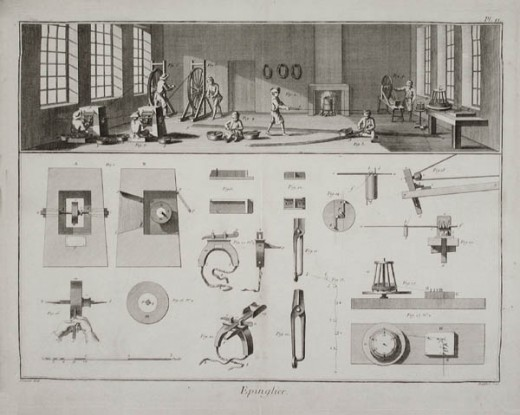
\includegraphics[width=6cm]{./img/adamsmith.jpg}
  \setlength{\abovecaptionskip}{0.5cm}
  \caption{Adam Smith's priknaaldfabriek}
\end{figure}

Intussen is meer dan duidelijk dat de taak van een BA kritiek is voor een effectieve
bedrijfsvoering. De bijhorende verloning wordt daarom ook bovengemiddeld ingeschat op
45 300 EUR, met als ondergrens 38 600 EUR en als bovengrens 55 400 EUR. Salarissen voor 
BA's buiten België liggen soms een stuk hoger, zoals in de VS, waar het 
gemiddelde boven de 80 000 USD ligt. \autocite{step} \autocite{howmuch}

BA's beheersen sowieso een tal van management gerelateerde vaardigheden, wat 
voor een zekere flexibiliteit zorgt op de arbeidsmarkt. Als BA is het daarom relatief eenvoudig 
om over te schakelen naar beroepen zoals project manager, econoom, IT manager, proces-coordinator 
enzovoort. Inhoudelijk sluit hun kennispakket ook goed aan op dat van andere analysefuncties, 
zoals die van data-analist, marketing-analist of functioneel analist. \autocite{bac1} \autocite{bac2}

Een BA is echter werkloos als zijn projectteam niet weet hoe ze aan de slag moeten. Er is nood
aan een gestandaardiseerde en effectieve manier van werken in development. Dit is de rol
die de agile methodiek tracht te spelen, bovenop het aanbrengen van drastische verbeteringen 
tegenover klassieke procedures zoals de watervalmethode. Bij agile wordt aan de hand van een
verzameling 'practices' de nadruk gelegd op korte iteraties en bijgevolg een hoge
behendigheid in het totale business proces. Enkele voorbeelden van deze practices zijn
onder andere version control en voortdurende demo's van de gevraagde oplossing bij de klant.
Agile combineert practices als deze op een unieke manier waarbij:
\begin{itemize}
  \item individuen/interacties boven processen/tools staan,
  \item werkende software boven concrete documentatie staat,
  \item samenwerking met de klant boven contractonderhandeling staat,
  \item en behendig ('agile') zijn boven het volgen van een plan staat.
\end{itemize}
Samenwerking en zelf-organisatie zijn sleutelwoorden in het Agile Manifesto. Projectteams
krijgen de vrijheid om zonder manager een geschikte uitwerking van de oplossing te bedenken.
Agile wordt niet aanschouwt als absoluut en staat variatie toe. Organisaties en teams die 
aan agile doen hebben vaak elk hun eigen interpretatie en uitvoering van de methodiek. \autocite{artagile}

Developers, ongeacht of ze agile werken of niet, staan soms twijfelachtig tegenover de 
samenwerking met een BA. Dit fenomeen vloeit voort uit het feit dat BA's in een brugpositie 
staan waarbij constante communicatie kritiek is - dit kan echter opgevat worden als 'controlerend'
of 'krampachtig' in het standpunt van een developer. Daarnaast zijn BA's onderworpen aan het 
feit dat ze regelmatig moeten 'gokken.' Dit is een normaal onderdeel van analyse, maar wanneer 
zo'n gok verkeerd ingeschat wordt kan dit voor frustraties zorgen bij projectteams. Sowieso 
schakelen BA's voortdurend tussen twee werelden: die van wat de klant graag zou wíllen 
krijgen en die van wat de klant kán krijgen. Deze constante wisselbeweging neemt zijn tol 
en zorgt ervoor dat sommige BA's een lagere stressbestendigheid ontwikkelen, wat de 
samenwerking met collega's verder bemoeilijkt. Developers klagen naast dit alles ook over 
hoe BA's regelmatig:
\begin{itemize}
  \item hen uit hun gedachteproces rukken,
  \item te veel vragen stellen in te weinig sessies,
  \item en onmogelijk korte deadlines voorschrijven.
\end{itemize}
\autocite{devba}

Al bij al tonen cijfers aan dat BA's ondanks de misnoegens toch een onmisbaar pluspunt zijn 
bij organisaties. Van bedrijven beweert 94\% dat vormen van analyse kritiek zijn voor hun
digitale bedrijfsvoering. Verder zegt 60\% van bedrijven wereldwijd dat ze vormen van 
analyse gebruiken om business processen te stroomlijnen. \autocite{stats}

Daarnaast wordt agile tegenwoordig aanschouwd als de standaard in de meeste bedrijven.
Van bedrijven werkt 71\% volgens de agile methodiek. De kans dat een agile project mislukt
wordt dan weer ingeschat op 8\%. \autocite{agilestats}

Bijgevolg kan geconcludeerd worden dat ongeveer 43\% van alle (software)bedrijven zowel BA's 
als agile benutten in hun werking. De rol van een BA in een agile werkomgeving wijzigt nochtans
niet opmerkelijk van die in een klassieke omgeving. Waar een BA vroeger in relatief grote stappen
requirements kon definiëren als onderdeel van een gevraagde oplossing, worden die stappen enkel
een stuk kleiner bij agile om zo behendigheid te kunnen garanderen. De rol van BA blijft 
ook bestaan als vertaalslag tussen de klant en het projectteam, met daar bovenop
dat BA's in agile soms de rol van 'product owner' ontvangen. Agile en subvormen ervan 
erkennen officieel niet het concept van een BA dus deze zal altijd één of meerdere gepaste 
rollen krijgen die toegestaan worden volgens de gebruikte methodiek. De product owner van 
een agile project is de persoon die verantwoordelijk is voor de requirements - een BA die deze rol
vervult zal dus niet enkel de requirements van een oplossing definiëren maar ook instaan voor
de succesvolle en correcte implementering ervan. Een ander voorbeeld van een agile rol die 
past bij de taak van een BA is die van de 'scrum master.' Hierbij spelen vooral soft skills 
van belang en worden bepaalde oorspronkelijke verantwoordelijkheden van de BA zelfs losgelaten. \autocite{agilebado} \autocite{nicole} \autocite{indian}
\begin{figure}[!ht]
  \centering
  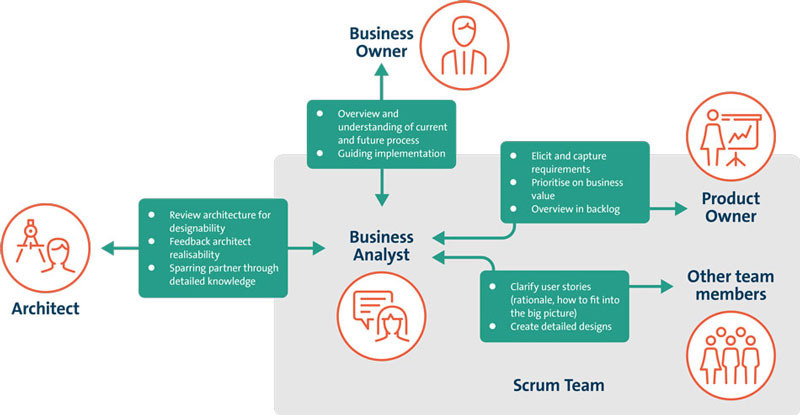
\includegraphics[width=8cm]{./img/agileBA.jpg}
  \setlength{\abovecaptionskip}{0.5cm}
  \caption{Een mogelijke aanpak van agile + BA}
\end{figure}

Terwijl de rol van een BA in agile grotendeels hetzelfde blijft, verandert in zijn werk wel 
het formaat, de technieken en zelfs de fysieke omgeving waarin het werk uitgevoerd wordt. 
Met 'requirements definiëren in kleine stappen' wordt bijvoorbeeld bedoeld dat BA's net zoals
agile projectteams volgens iteraties moeten werken. Dit geldt ook voor de analyse zelf.
Als resultaat hiervan is een agile BA voor de volledige duur van een agile project betrokken,
terwijl bij klassieke werkmethodes de BA, zodra zijn taak erop zat, als eerste het project 
verliet. Een andere aanpassing waar BA's in agile onderhevig aan zijn is dat ze niet meer (fysiek)
geïsoleerd kunnen werken - ze worden namelijk onderdeel van een communicatief, voortdurend
bewegend team. Daarnaast verdwijnt in agile een groot deel van de analyse-documentatie, iets waar 
een BA zich traditioneel met bezig hield. Normaliter werd een requirements document uitgeschreven, 
wat bij agile niet meer het geval is. In plaats daarvan voorziet een BA zijn projectteam verbaal 
of zelfs informeel van de gevraagde producteigenschappen. Dit gebeurt dan onder andere in de 
vorm van user stories. \textbf{Voor een BA in agile ligt de focus liever op concreet inzicht 
verwekken in de probleemstelling dan op uitgebreide documentatie uitschrijven. Een BA in een 
agile werkomgeving weet dat zijn taak geslaagd is als zijn projectteam perfect weet waarom 
er een bepaalde requirement is en waarom een bepaalde requirement plots wijzigt of verdwijnt.} Wat mede helpt bij het bereiken van dit doeleinde is een divers 
projectteam dat bestaat uit mensen met verscheidene technische achtergronden. Er wordt op deze
manier sneller een consensus bereikt over de precieze aard van het probleemdomein. \autocite{expertagile}

\section{Interviews}

Om buiten de literatuurstudie een meer concrete inkijk te verwerven in hoe organisaties
business analists inzetten bij agile development teams, werden verscheidene
interviews afgenomen, zowel fysiek als telefonisch. Antwoorden van de geïnterviewden werden 
schriftelijk vastgelegd waardoor ze licht kunnen verschillen van de werkelijkheid op grond
van grammaticale verbeteringen. De geïnterviewden gaven allemaal vooraf verbale 
toestemming om hun naam, werkplaats en antwoorden te laten noteren en delen met Hogeschool Gent. 

\subsection{Algemene vragenlijst}

Onderstaand het inspiratiemateriaal voor de afgenomen interviews. Sommige vragen werden vervormd
tijdens de gesprekken om zo beter in te kunnen gaan op het voorgaande antwoord van de geïnterviewde.

\vspace{5pt}

\begin{enumerate}[label=\bfseries\Alph* |]
  \item Een kleine introductie; wat is uw functie op uw huidige werkplaats?
  \item Hoe gaan jullie om met de analyse voor softwareprojecten? Beschikken jullie over een business analist of gelijkaardige rol?
  \item Doen of deden jullie ooit aan agile development? Hoe groot zijn de projectteams? 
  \item Hebben agile projectteams rechtstreeks contact met de klant of is de business analist het schakelpunt?
  \item Is de product owner van een agile project de business analist of zit dat anders? Wordt de business analist überhaupt aanschouwt als deel van het projectteam?
  \item Denkt u dat business analisten meer of minder werk hebben met agile projecten tegenover andere werkmethoden?
  \item Heeft u voorbeelden van een geslaagd en/of mislukt project ter gevolge van de analyse?
  \item Verloopt de samenwerking tussen business analists en agile projectteams vlot? Wat zijn veelvoorkomende struikelblokken?
  \item Soft skills zijn kritiek voor een goede analist. Wat zijn naar uw ervaring de drie belangrijkste?
  \item Zou agile development zonder een business analist kunnen? Hoe zouden zulke projecten performeren?
  \item Aan gemiddeld hoeveel projecten tegelijkertijd is een business analist bezig, of werken ze één per één?
  \item Is het meestal de klant of de business analist die contactmomenten initieert, of varieert dat?
  \item Wat is het slechtste dat een business analist kan doen? Heeft u die situatie ooit al meegemaakt?
  \item Agile development en business analyse worden tegenwoordig nogal verhemeld. Denkt u dat dit terecht is of wordt er overdreven?
  \item Denkt u dat business analyse een goede arbeidsmarkt heeft? Wordt hun rol belangrijker of net niet?
\end{enumerate}
 
\subsection{Dhr. Dieter Vanthorre (Dana)}
\textsc{\underline{Dit interview werd op afstand afgenomen}}

\vspace{5pt}

Dana (www.dana.com) is wereldwijd een voorloper op gebied van zowel elektrische als conventionele aandrijflijnen.
Met een focus op technisch-mechanische aspecten gaat hier echter ook een IT-afdeling aan de slag, met als aanvoerder Dieter Vanthorre.
In zijn team zijn drie business analisten actief: 

\begin{itemize}
  \item een analist die werkt voor engineering-applicaties,
  \item een analist die werkt voor shop floor-applicaties,
  \item en een ERP-analist die werkt met AS 400.
\end{itemize}
Bij projectmatig werken vindt de oorsprong van de opdracht zich consistent bij hoger management. Bij momenten van stilstand
richt Vanthorre zijn team op de kleinere break/fix-taken. Qua methodiek wat betreft deze projecten is er volgens Vanthorre
meestal sprake van het watervalsysteem, maar wanneer het project als groot genoeg wordt aanschouwd werkt men met agile.
Deze classificatie is echter dynamisch - een watervalproject kan tijdens de uitvoering worden omgezet naar een agile project
indien de scope voldoende toeneemt. Een ander fenomeen is dat, vooral tijdens en na voornoemde overgangsfase, de analyse-functie van de BA
door ieder lid van het projectteam gedragen wordt. Omwille de kleine omvang van de (agile) projectteams wordt de rol van een BA 
gezien als de verantwoordelijkheid van elk projectlid.

Daarnaast is er bij agile sprake van weinig documentatie, maar bij Dana worden ook bij watervalprojecten weinig zaken schriftelijk 
vastgelegd. Vanthorre vermeldt dat de meeste communicatie mondeling verloopt.

\subsection{Dhr. Ignace Maes (OTA Insight)}
\textsc{\underline{Dit interview werd op afstand afgenomen}}

\vspace{5pt}

OTA Insight (www.otainsight.com) is in vergelijking met Dana een stuk groter. Als SAAS-ontwikkelaar is men er voornamelijk bezig met
het ontwikkelen van BI-applicaties. Ignace Maes, full-stack developer bij OTA Insight, is deel van één van hun vele development teams.
Maes vertelt dat bij OTA Insight exclusief gewerkt wordt volgens agile. Daarnaast is het tribe-systeem er ook actief.

Op gebied van business analyse is de bijhorende rol vooral actief bij solution architects en product managers. Deze twee functies
houden zich echter niet énkel bezig met business analyse - hier dient deze als basis waarop het respectievelijke takenpakket verder wordt uitgebreid.
Een solution architect is bijvoorbeeld naast zijn analytische functie ook engineer, verantwoordelijk voor het uitwerken van het technische
plan voor een project aan de hand van geobserveerde requirements. Een product manager aan de andere kant zal als bijhorend takenpakket
minder technische aspecten behandelen. Hun taak is qua business analyse zuiverder: ze verzorgen de communicatie met stakeholders en werken
product en/of requirements conceptueel uit. Al snel is duidelijk dat het vooral de product managers zijn die de product backlog 
opbouwen.

Wat betreft documentatie neemt OTA Insight zaken erg serieus, zegt Maes. Er is bij het documentatieproces van een product sprake van drie fases:

\begin{enumerate}
  \item een algemene omschrijving wordt uitgewerkt,
  \item de details worden verder uitgewerkt,
  \item alles nagekeken door zowel engineers als developers.
\end{enumerate}
Ook wordt vermeldt dat het belang van analyse bij OTA Insight aanzienlijk is toegenomen sinds de explosieve groei van het bedrijf, wat
alsook geldt voor hun documentatieproces. 

Volgens Maes wordt business analyse meer en meer een verantwoordelijkheid
van ieder projectlid en niet enkel een aangewezen BA. Solution architects en product managers ervaren dit het sterktst, maar ook de 'gewone'
developer draagt zijn steentje bij wat betreft de analyse.

\subsection{Dhr. Wim Vervust (Refleqt)}
\textsc{\underline{Dit interview werd fysiek afgenomen}}

\vspace{5pt}

Refleqt (www.refleqt.be) bevindt zich in het milieu van IT-consultancy en legt de nadruk graag op testautomatisatie. Wim Vervust is één van de twee
oprichters en heeft een managementspositie (Quality Coach) waarbij hij vooral verantwoordelijk is voor de end-to-end oplevering van projecten.

Bij Refleqt wordt de rol van BA aangenomen door de zogenaamde 'Functionele Lead.' Deze is zowel actief bij projecten die agile als traditioneel
tewerk gaan. Vervust en de teams verkiezen agile, maar maken duidelijk dat dit niet altijd mogelijk is. Een klant kan bijvoorbeeld uitdrukkelijk wensen niét agile 
te gebruiken, of de inhoud van het project kent geen vooruitschrijdende aard waardoor ze niet compatibel is met deze werkmethode.

De functionele lead wordt aanschouwd als vast onderdeel van het projectteam, maar zijn taak wordt minder kritiek naarmate het project de eindstreep nadert - een typerende
eigenschap van de analyse. Het gebeurt dan soms ook dat deze persoon al aan een ander, opstartend project wordt toegewezen van zodra de werklast vermindert. Het feit dat men bij Refleqt agile 
werkt neutraliseert dit effect gedeeltelijk - één groot lastenboek opstellen aan het begin van het project gebeurt dan ook niet meer en de BA blijft langer  een
actieve rol spelen in het projectteam. Vervust zegt dat het grootste verschil tussen agile en klassieke werkmethodes is dat het bij agile vrijwel onmogelijk
is om een volledig overzicht te krijgen. Bij Refleqt zal een BA in een agile project daarom niet noodzakelijk meer werk hebben, maar wel anders tewerk moeten gaan.

Verder wordt duidelijk gemaakt dat een project zonder analyse onmogelijk is. Bij de afwezigheid van een BA zal de rol altijd elders vervuld worden. In de praktijk
is dit dan meestal het projectlid met de meeste ervaring. Sowieso zal de vraag naar analisten voorlopig blijven stijgen, evenredig met hoe de vraag naar ontwikkelaars 
groeit. De verhouding hiertussen blijft onveranderd, ondanks het feit dat de taak van analisten complexer wordt.

\section{Conclusies}

Bij business analyse in agile werkomgevingen ligt de nadruk op het verwekken van inzicht in het probleemdomein. Documentatie valt
op tweede prioriteit (nice-to-have) - men wil eerst en vooral bereiken dat elk lid van het projectteam op dezelfde golflengte zit wat betreft de 
precieze aard van het gewenste product. Het is bij agile van belang dat er sprake is van flexibiliteit naar de wensen van de klant toe, wat de taak van een BA
(als die er überhaupt is) dynamischer maakt t.o.v. traditionele werkmethodes.

Daarnaast valt een concreet toegewezen BA in agile teams geregeld compleet weg en wordt de analyse in zulke gevallen
een gezamenlijke verantwoordelijkheid binnenin het projectteam. Sowieso moet opgemerkt worden dat business analyse in agile niet zozeer een 
vaste functietoewijzing kent, maar eerder een pseudo-rol is die op één of andere manier moet vervuld worden. Het aanspreekpunt voor de klant wordt in deze
situaties mondeling overeengekomen of wordt doorgeschoven naar een andere rol, zoals de product owner.

Alsook vastgesteld is dat bij de groei van een bedrijf het belang van de analyse minstens evenredig toeneemt. Wat echter niet verandert is dat de klant
in ieder geval centraal blijft staan - bij agile zal enkel de mate, manier en frequentie van communicatie tussen stakeholder en analist veranderen.

%------------------------------------------------------------------------------
% Referentielijst
%------------------------------------------------------------------------------

\phantomsection
\printbibliography[heading=bibintoc]

\end{document}